\chapter{Fourier-Theorie f"ur die Kugeloberfl"ache\label{chapter:kugel}}
\lhead{Fourier f"ur die Kugeloberfl"ache}
\begin{refsection}
\chapterauthor{Thomas Gujer und Christoph Schmitz-Dr"ager}



\section{Einleitung}
\rhead{Einleitung}

In diesem Kapitel wollen wir die Gemeinsamkeiten und Unterschiede zwischen der klassischen Fourier-Theorie und der Fourier-Theorie auf der Kugeloberfl"ache aufzeigen.
 

\section{Kugelaufbau}
\rhead{Kugelaufbau}

\begin{figure}%Bild Koordinaten der Kugel
\centering
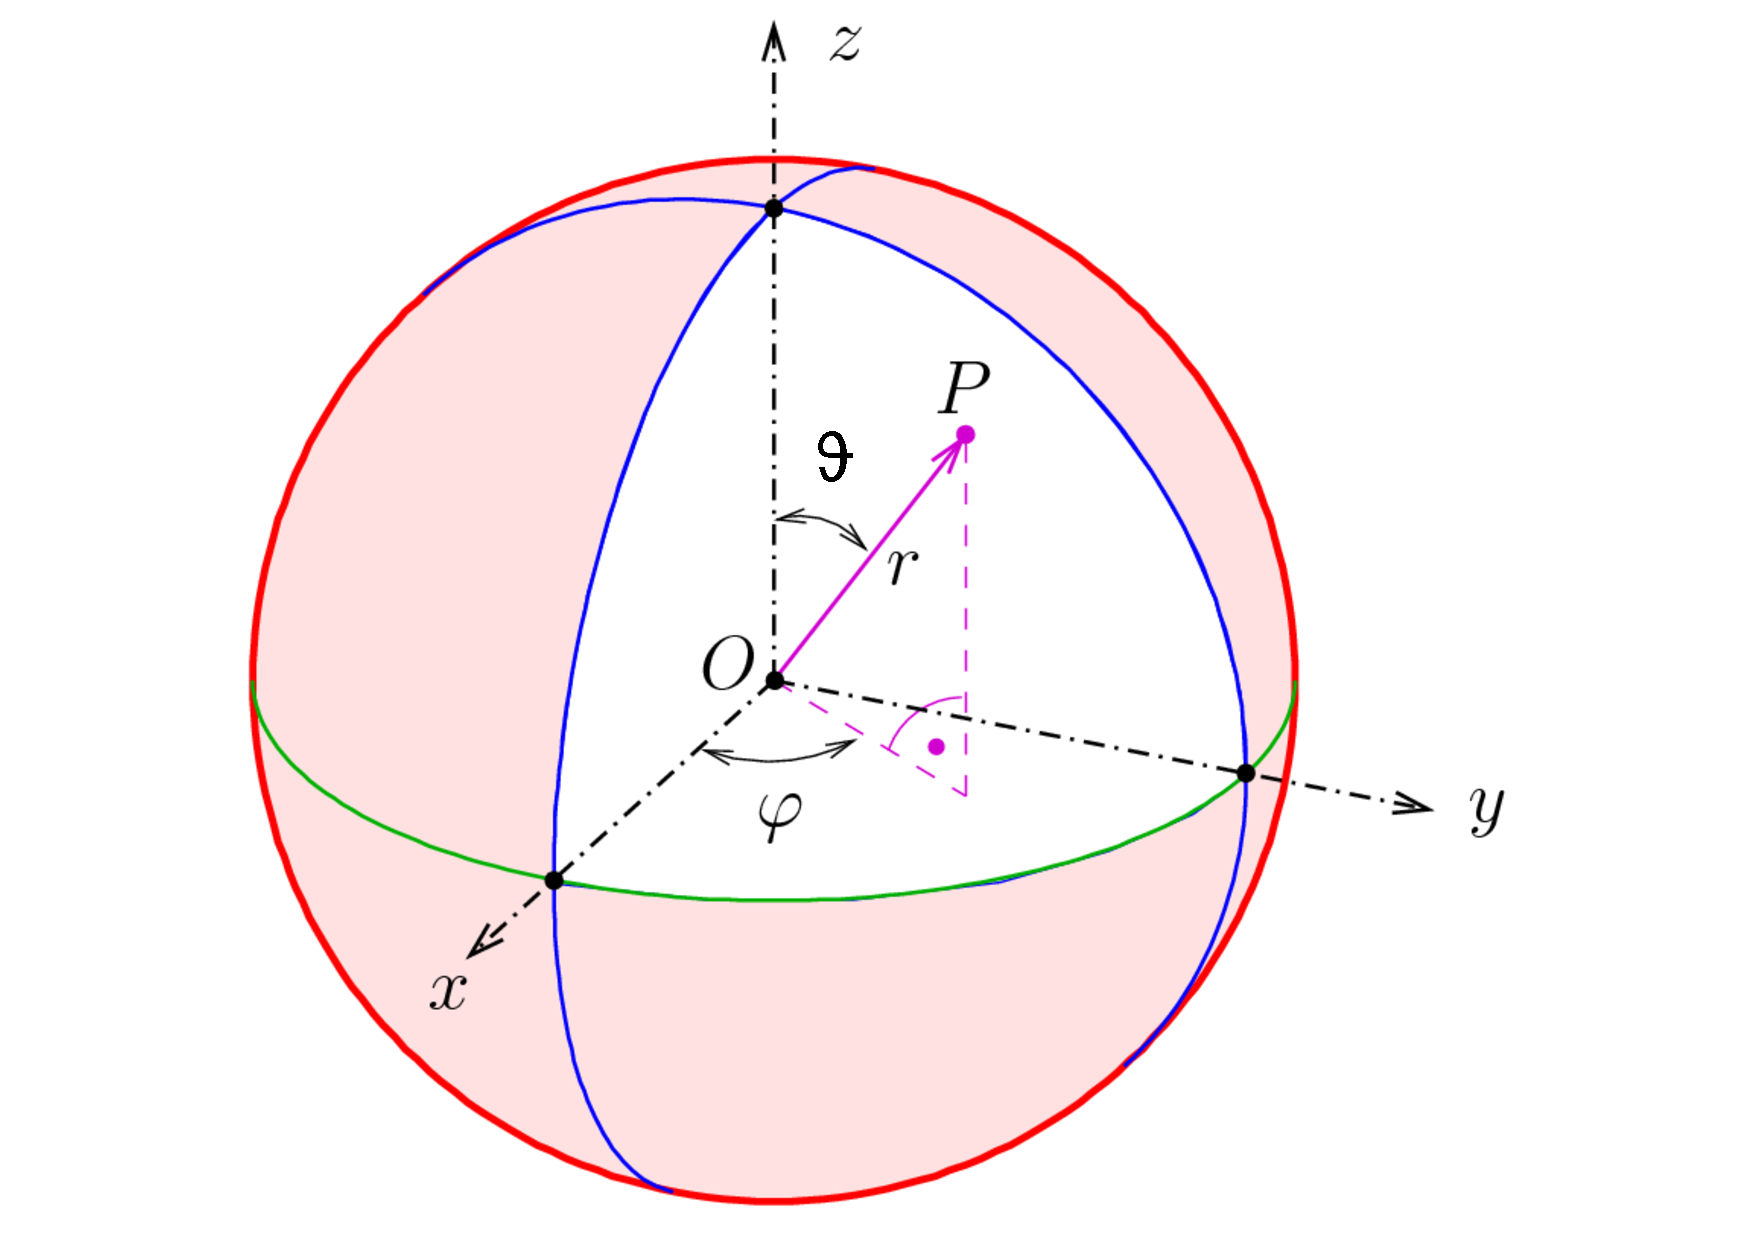
\includegraphics[width=0.7\textwidth]{kugel/Kugelkoord.pdf}
\caption{Koordinaten der Kugel
\label{skript:Koordinaten der Kugel}}
\end{figure}

In der Abbildung~\ref{skript:Koordinaten der Kugel}   
ist zu sehen wie ein Punkt auf der Kugeloberfl"ache im Polar-Koordinaten definiert ist. Zum umrechnen ins kartesische Koordinatensystem werden folgende Formeln ben"otigt:
\begin{align*}
x& = r \cdot sin(\vartheta) \cdot cos(\varphi) 
\\
y& = r \cdot sin(\vartheta) \cdot sin(\vartheta)
\\
z& = r \cdot cos(\vartheta) 
\end{align*}
 
 
\section{Aufbau der Funktion}
\rhead{Aufbau der Funktion}

\begin{figure}%Funktion auf Rechteckoberfläche 
\centering
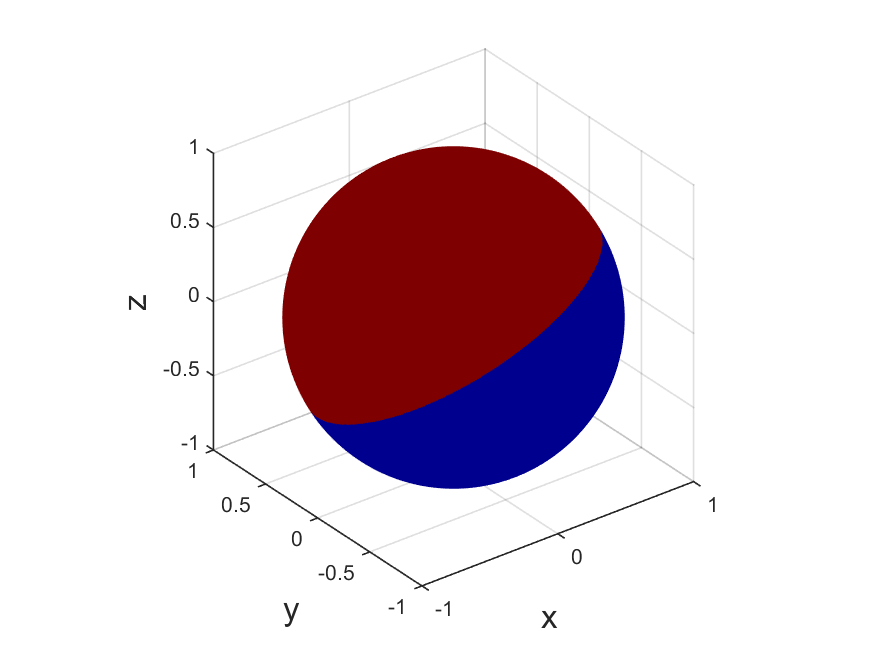
\includegraphics[width=0.7\textwidth]{kugel/Funktion.pdf}
\caption{Funktion auf Rechteckoberfl"ache
\label{skript:Koordinaten der Kugel}}
\end{figure}

Es wird mit einer Funktion gearbeitet, welche 3 Inputvariablen $f(x;y;z)$ bzw. $f(r;\vartheta;\varphi$) und eine Output Variable besitzt. Der Radius ist in unserem Fall konstant = 1 das wir uns nur auf die Kugeloberfl"ache beziehen. Das Ziel ist, auf der Kugeloberfl"ache einem kreisf"ormigen Abschnitt den Wert 1 und dem Rest der Kugeloberfl"ache den Wert 0 zuzuweisen. Geometrisch (in der 3-dimensionalen Betrachtung) "andert sich die Kugel nicht. Die Output Variable kann nur noch mit Farben dargestellt werden. Es ist dieselbe Darstellung, welche z.B. auch für die Temperatur auf der Erdoberfl"ache verwendet wird. In diesem Fall sollte man die Form der Erde auch nicht beeinflussen um die Temperatur darzustellen. Deshalb verwendet man einen Farbschl"ussel f"ur die Darstellung der verschiedenen Temperaturen.\\

Die Funktion in diesem Kapitel wurde folgendermassen definiert:\\
\begin{enumerate}


\item Definition eines Vektors mit dem Startpunkt im Zentrum der Kugel und dem Endpunkt in einem Punkt auf der Kugeloberfl"ache:

$$
\vec{c} = 
\begin{pmatrix}
r\\
\vartheta\\
\varphi
\end{pmatrix}
\text{mit r = 1 folgt}
\begin{pmatrix}
1\\
\vartheta\\
\varphi
\end{pmatrix}
$$

\item	Des Weiteren wird ein Vektor definiert, welcher den Startpunkt im Zentrum der Kugel und den Endpunkt auf der Kugeloberfl"ache hat. Im Gegensatz zum $\vec{c}$ wo die Winkel $\vartheta$ und $\varphi$ eindeutig definiert sind besitzt der $\vec{r}$ ein variables $\vartheta$ von 0 bis $\pi$ und ein variables $\pi$ von $-\pi$ bis $\pi$: \\

$$
\vec{r} = 
\begin{pmatrix}
r\\
\vartheta\\
\varphi
\end{pmatrix} 
$$\\

\item $\vec{c}$ und  Vektorenschar $\vec{r}$ in kartesische Koordinaten umrechnen\\

\item
\[
f(x;y;z) =\begin{cases}
1& \qquad \text{wenn C $\circ$ R $\ge$ 0 (Beispiel Halbkugel)}\\
0& \qquad \text{sonst}
\end{cases}
\]


\end{enumerate}
\section{Kugelfl"achenfunktionen}
\rhead{Kugelfl"achenfunktionen}


\begin{figure}% Bilder 0-2 Y_lm und Z_lm
\centering
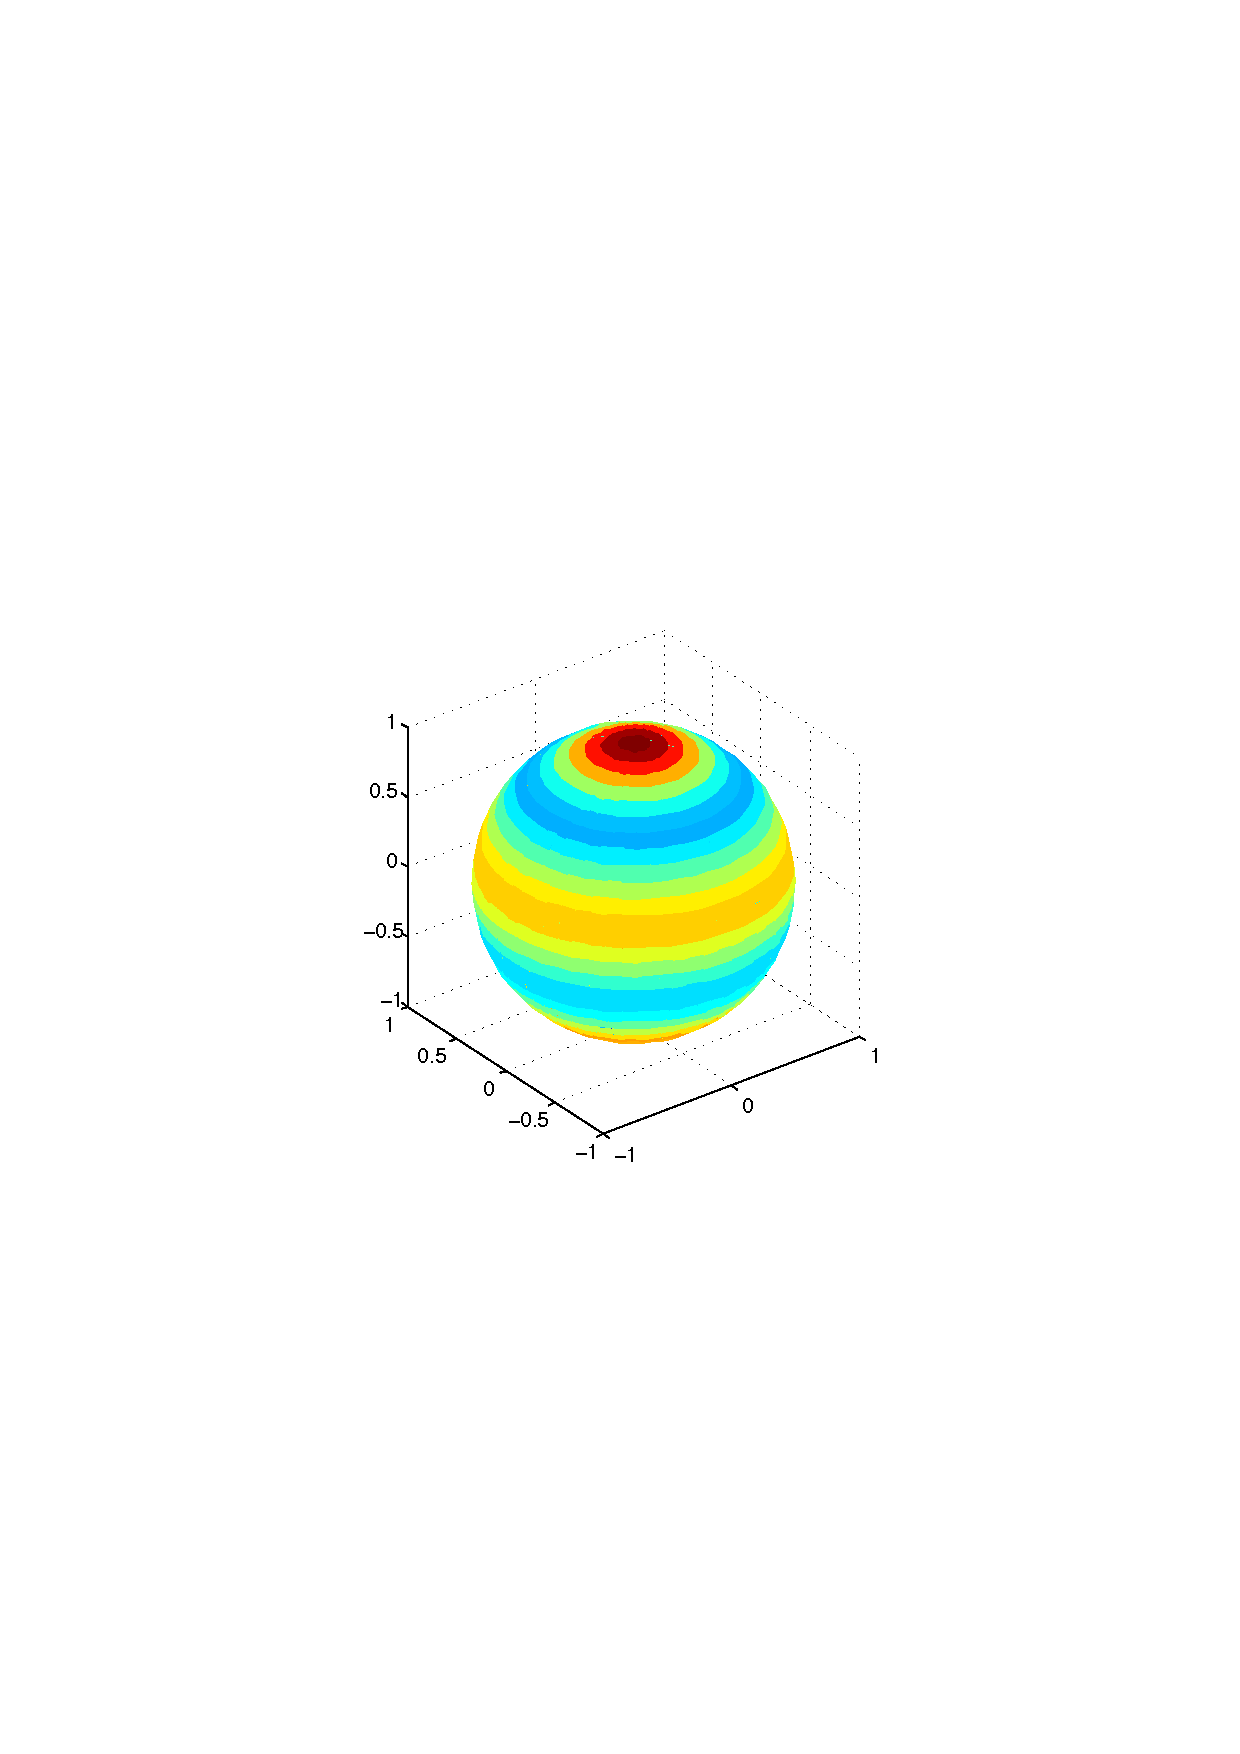
\includegraphics[width=0.45\textwidth]{kugel/ylm/a_5_0.pdf}
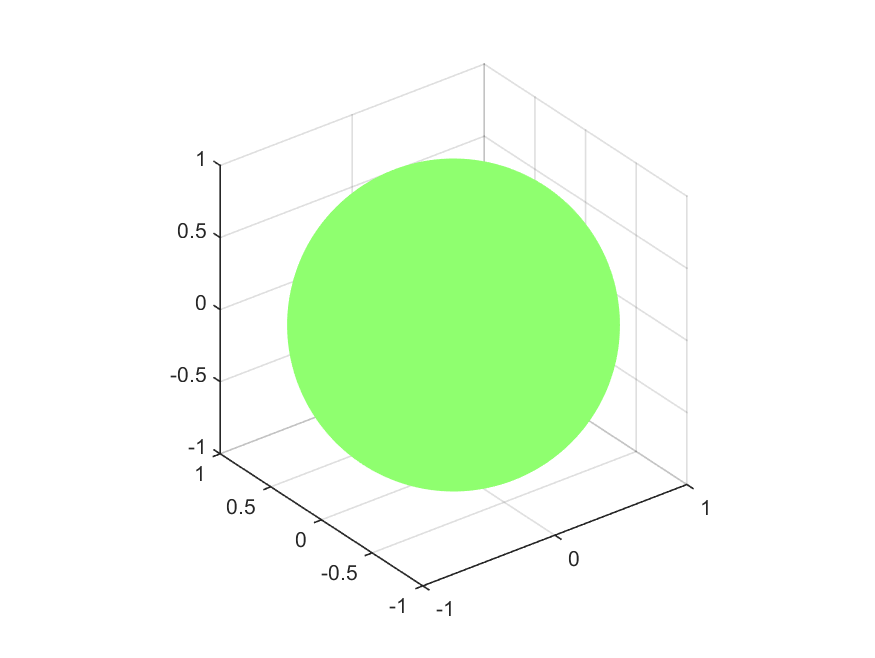
\includegraphics[width=0.45\textwidth]{kugel/ylm/b_5_0.pdf}
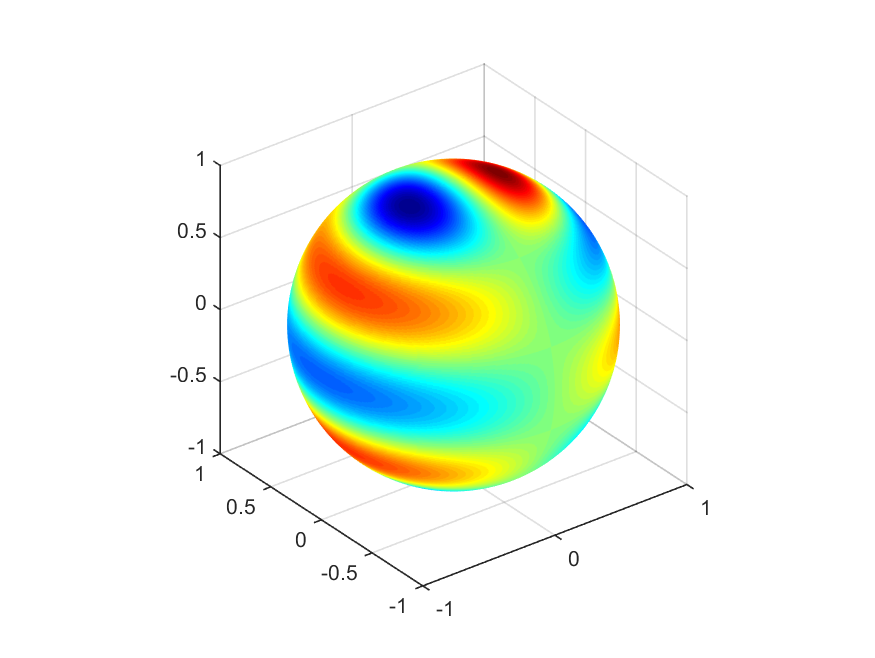
\includegraphics[width=0.45\textwidth]{kugel/ylm/a_5_1.pdf}
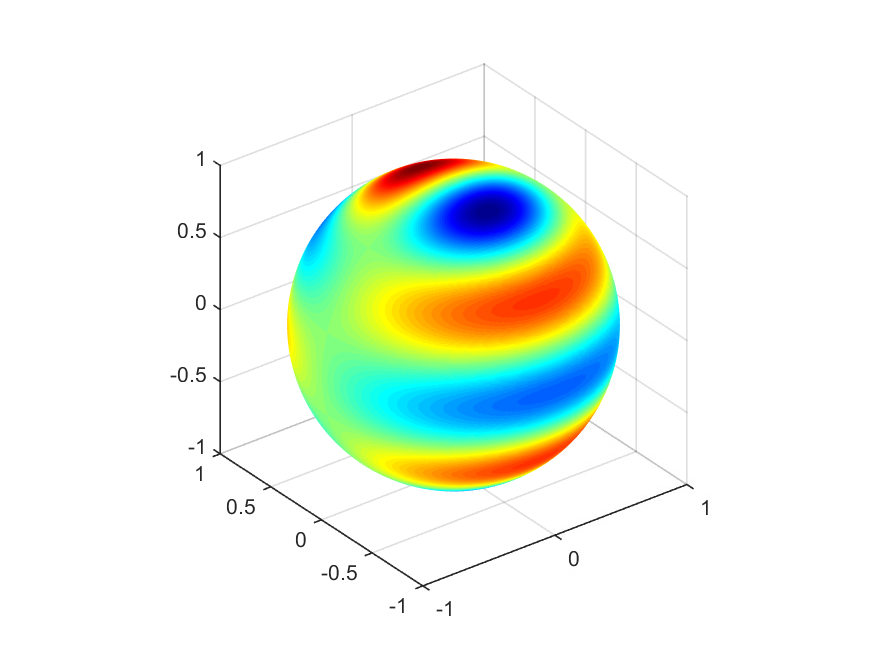
\includegraphics[width=0.45\textwidth]{kugel/ylm/b_5_1.pdf}
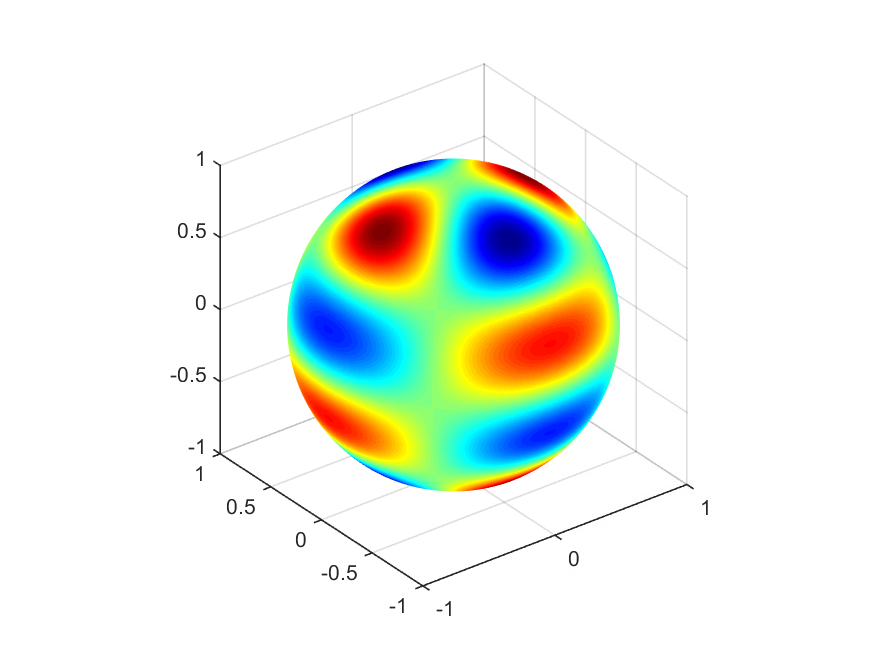
\includegraphics[width=0.45\textwidth]{kugel/ylm/a_5_2.pdf}
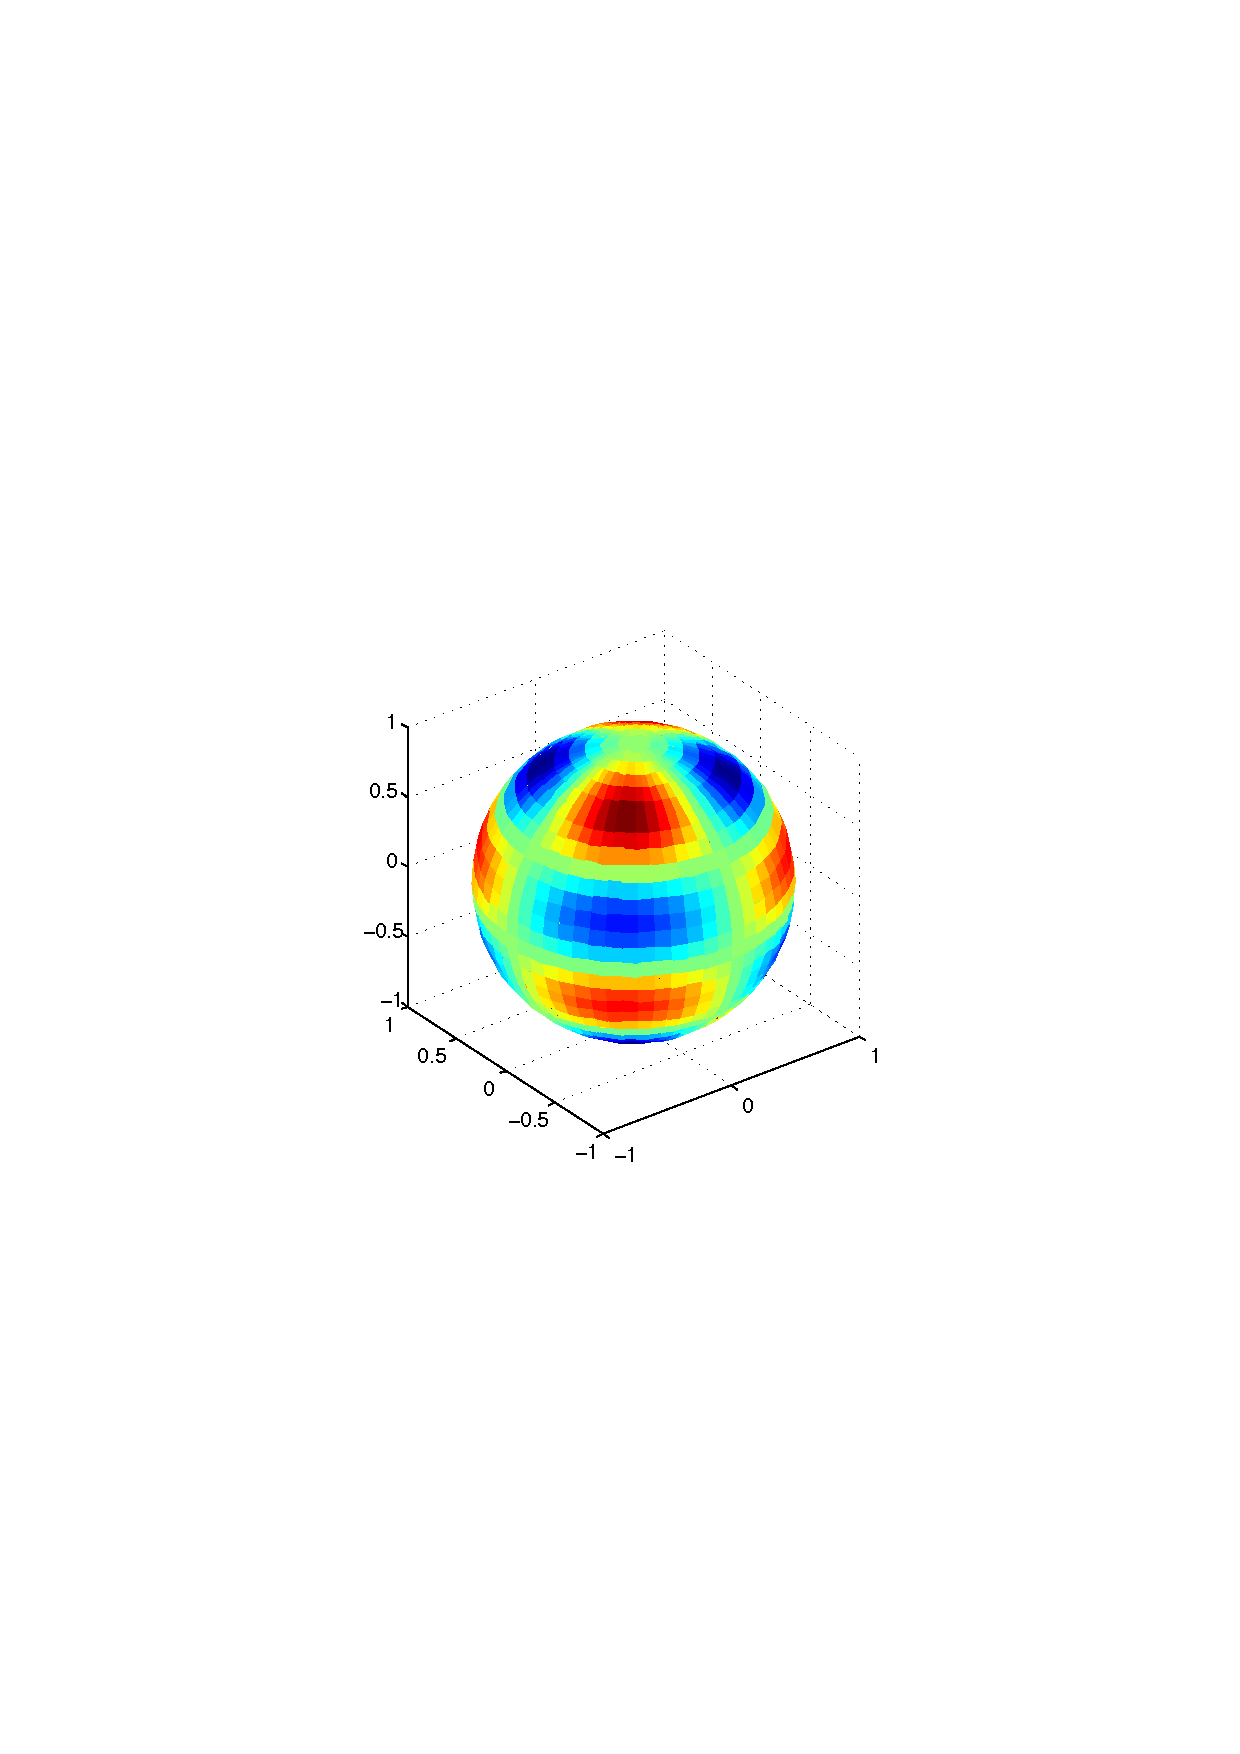
\includegraphics[width=0.45\textwidth]{kugel/ylm/b_5_2.pdf}
\caption{$Y_{lm}$ mit $l=5$, $m=0$, 1, 2 $\&$ $Z_{lm}$ mit $l=5$, $m=0$, 1, 2
\label{skript:Bild 0}}
\end{figure}

\begin{figure}% Bilder 3-5 Y_lm und Z_lm
\centering
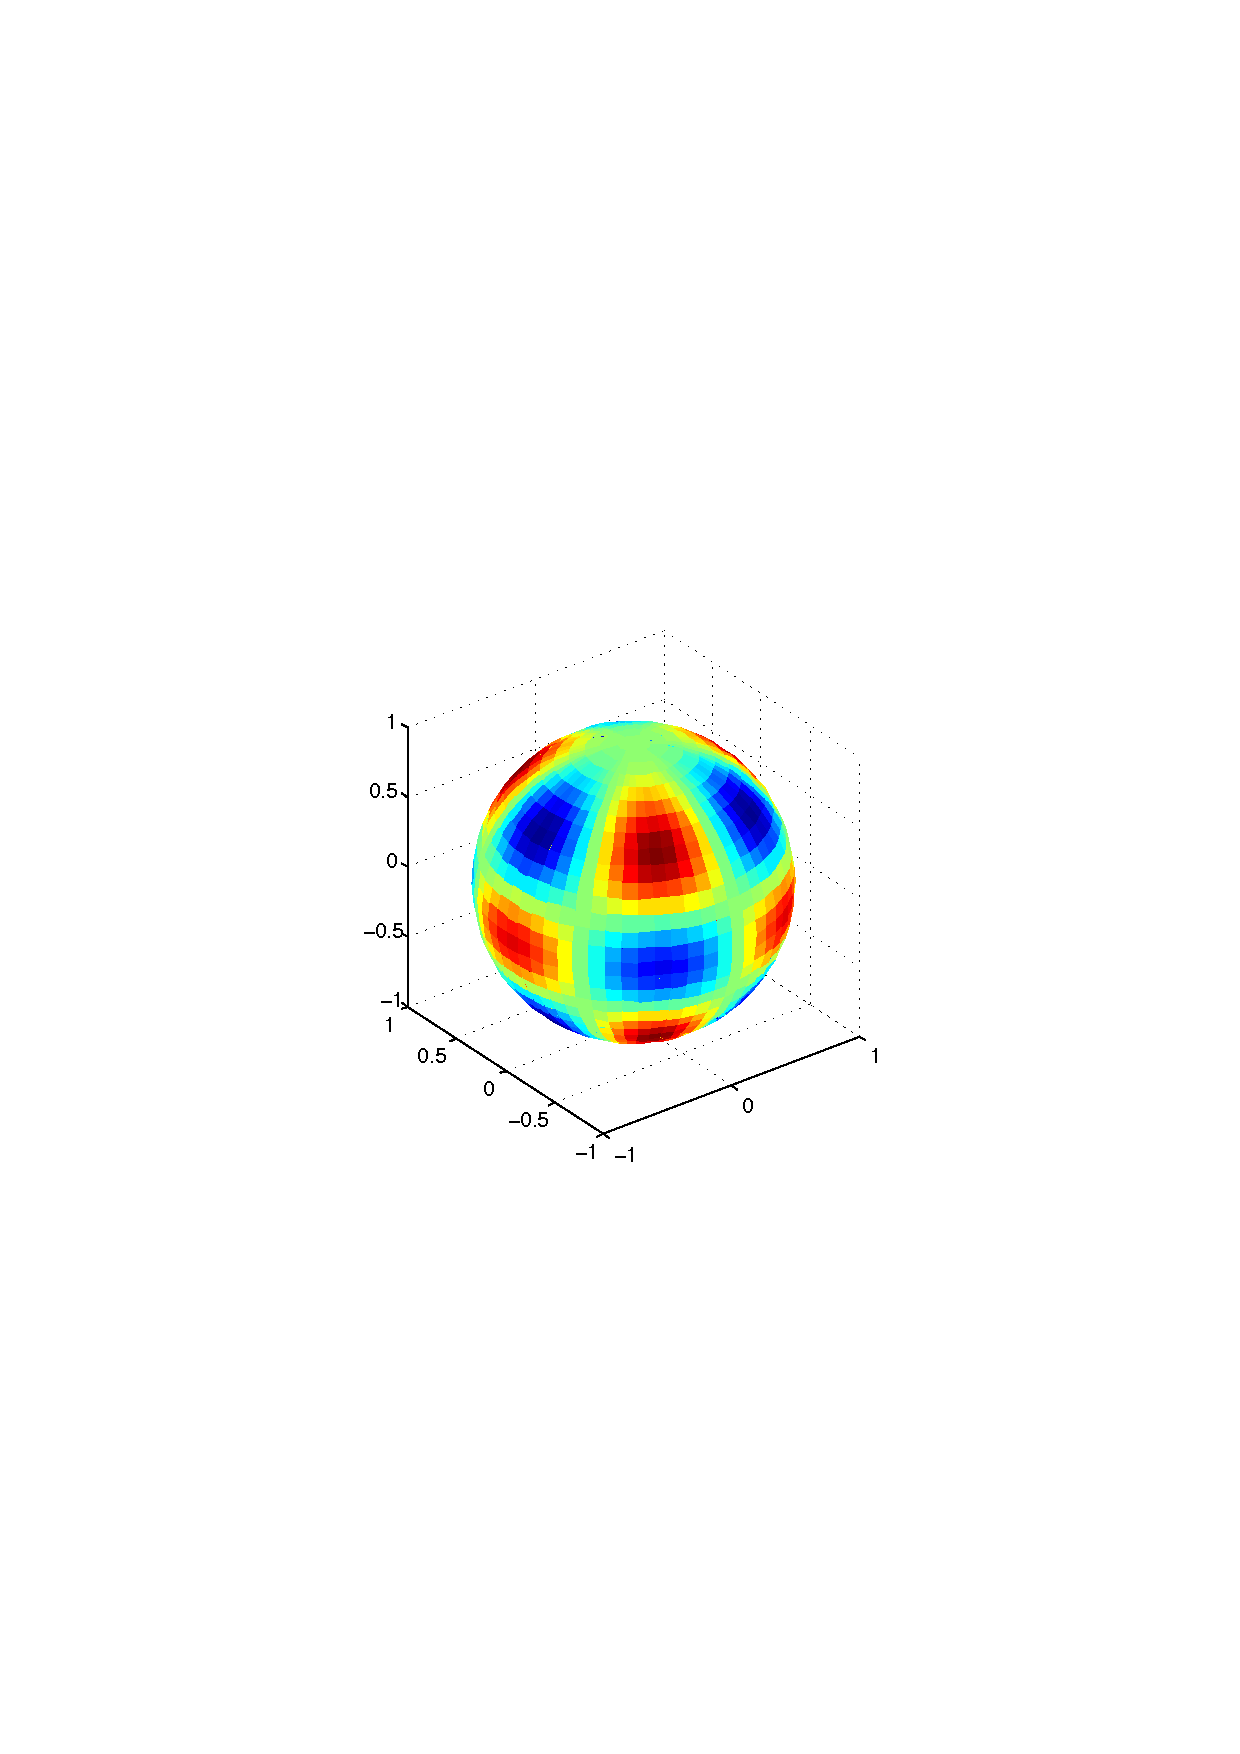
\includegraphics[width=0.45\textwidth]{kugel/ylm/a_5_3.pdf}
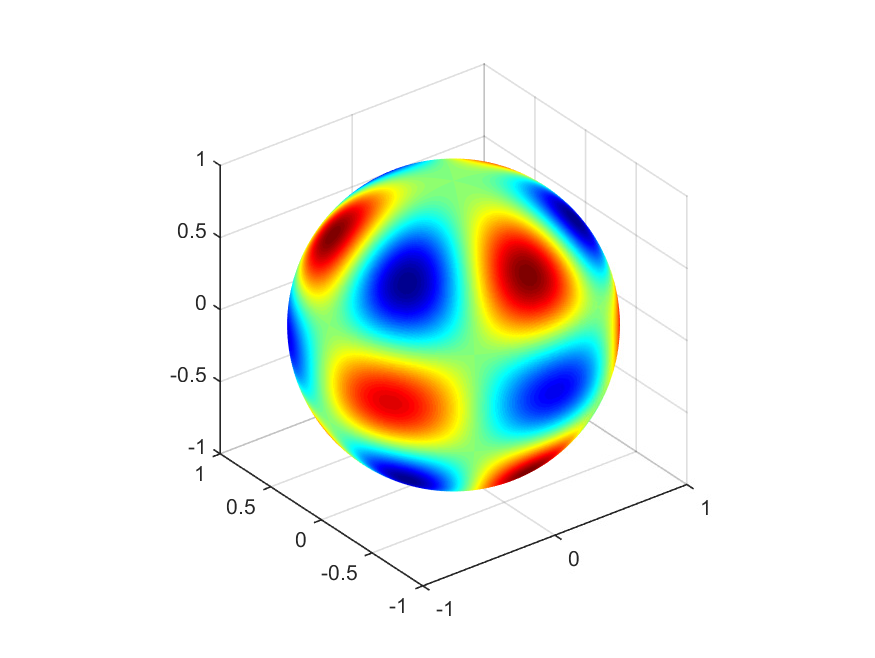
\includegraphics[width=0.45\textwidth]{kugel/ylm/b_5_3.pdf}
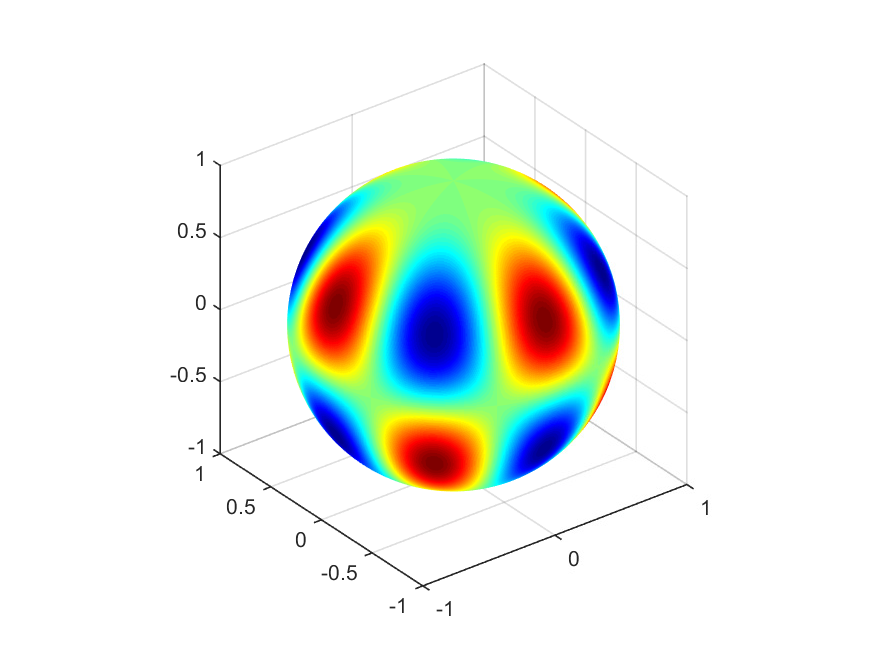
\includegraphics[width=0.45\textwidth]{kugel/ylm/a_5_4.pdf}
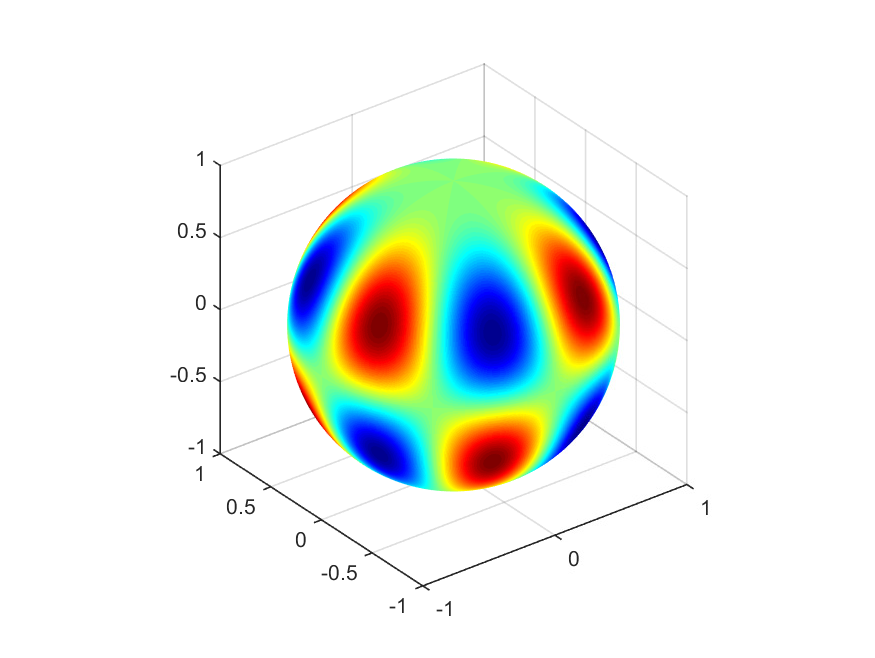
\includegraphics[width=0.45\textwidth]{kugel/ylm/b_5_4.pdf}
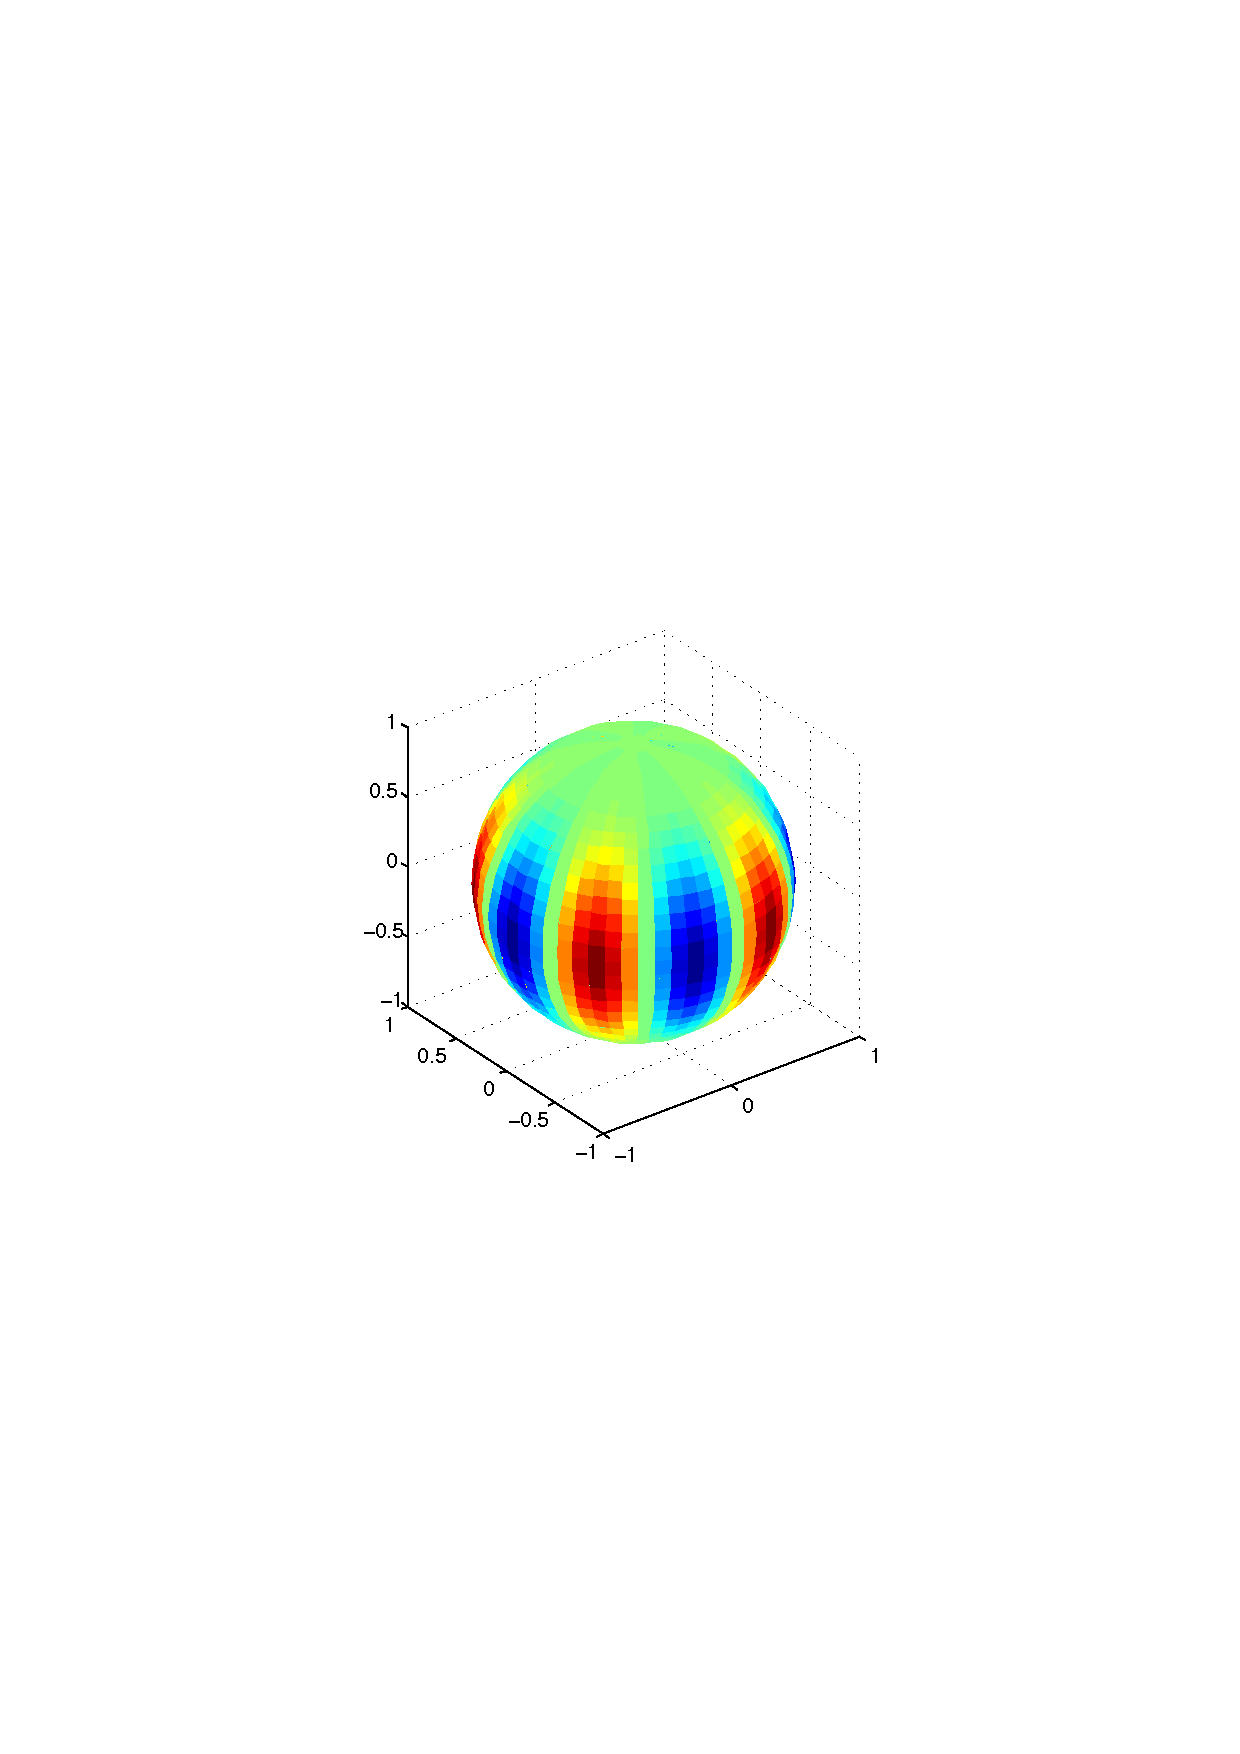
\includegraphics[width=0.45\textwidth]{kugel/ylm/a_5_5.pdf}
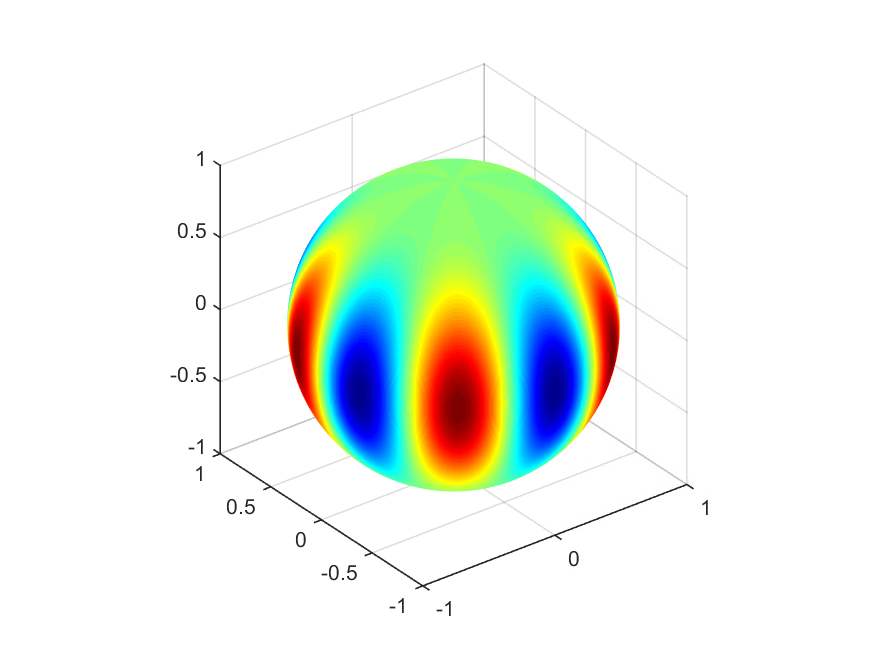
\includegraphics[width=0.45\textwidth]{kugel/ylm/b_5_5.pdf}
\caption{$Y_{lm}$ mit $l=5$, $m=3$, 4, 5 $\&$ $Z_{lm}$ mit $l=5$, $m=3$, 4, 5
\label{skript:Bild 2}}
\end{figure}

\section{Gibbsscher-Effekt} 
\rhead{Gibbsscher-Effekt}

\begin{figure}% Gibbsscher-Effekt
\centering
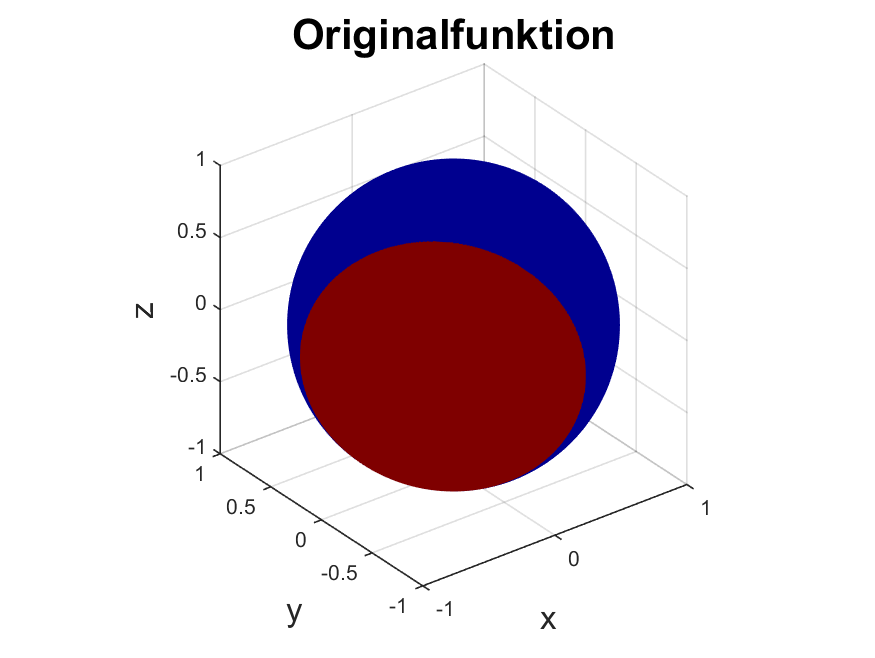
\includegraphics[width=0.4\textwidth]{kugel/Gibbs/GibbsOriginalFunktion.pdf}
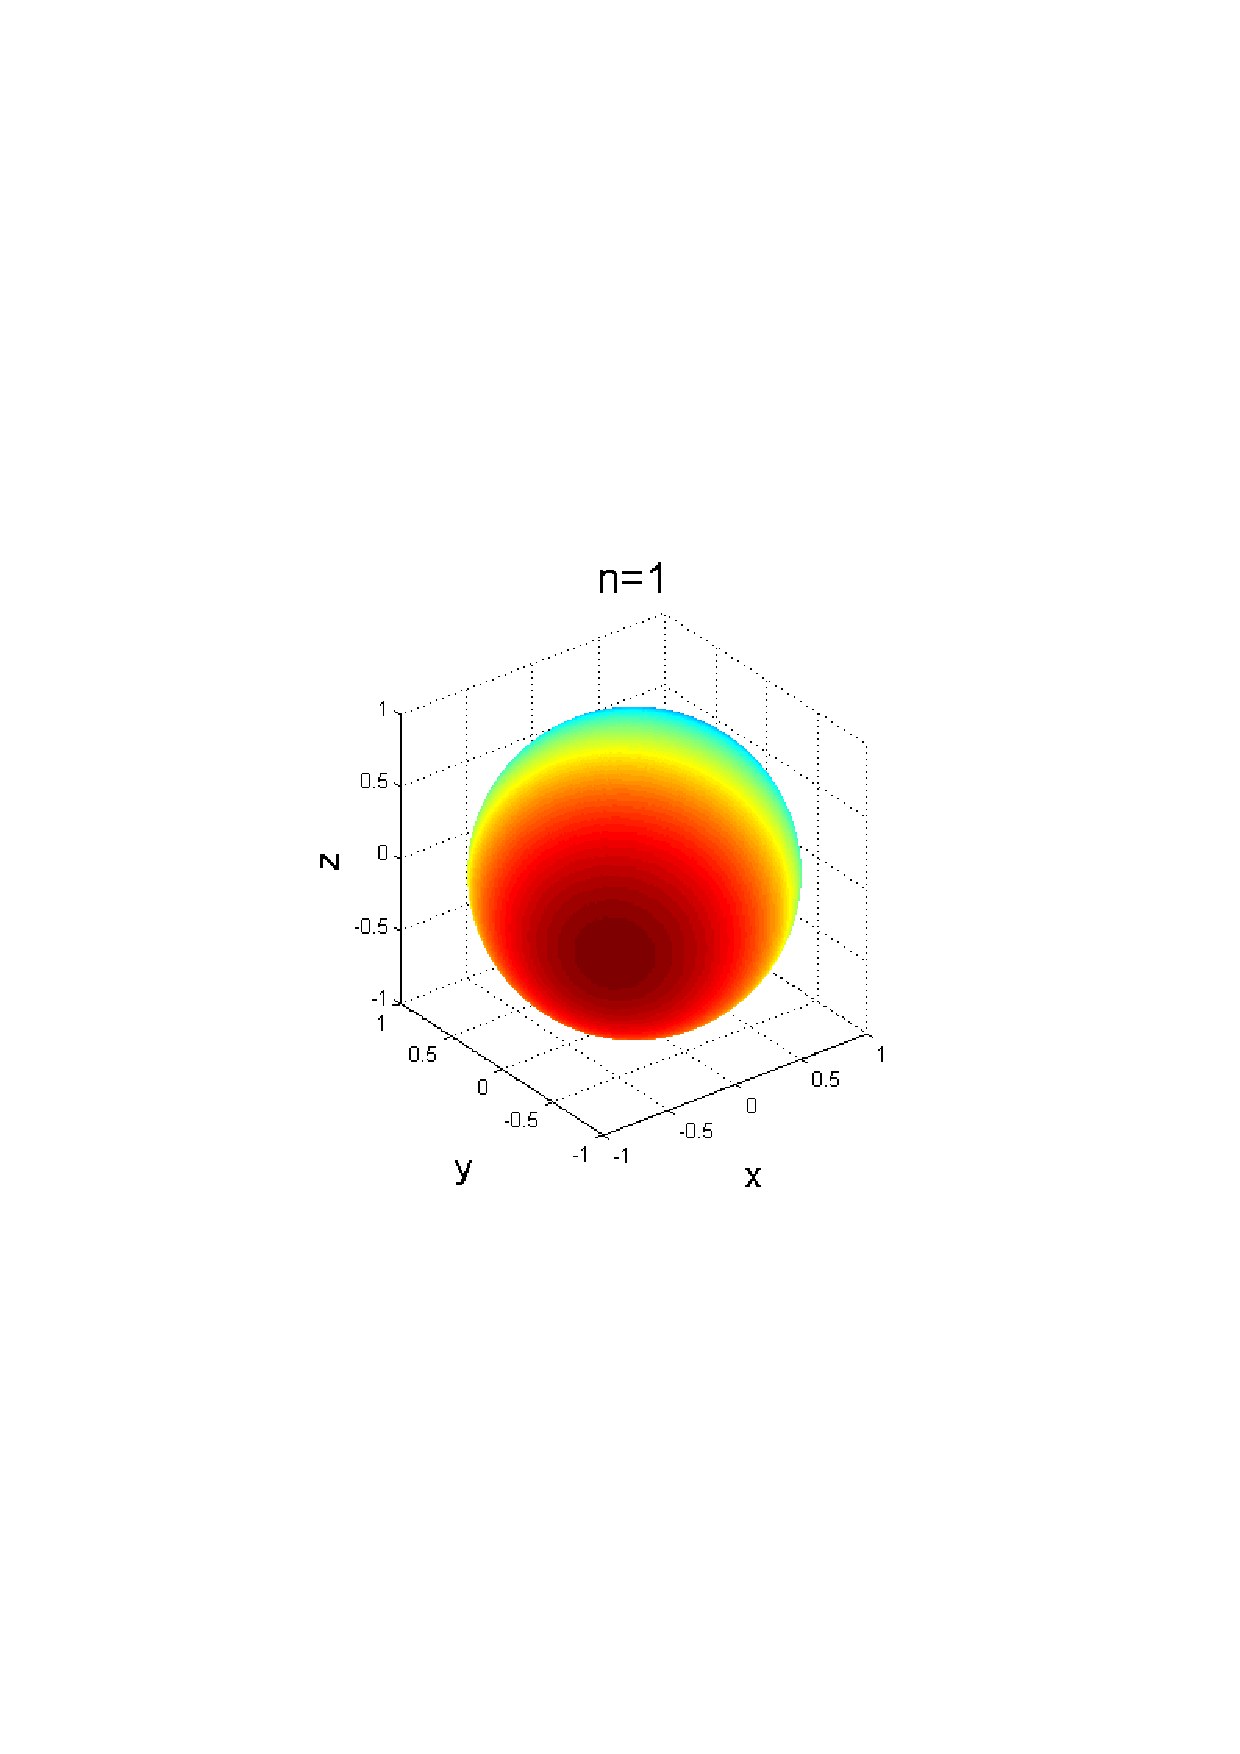
\includegraphics[width=0.4\textwidth]{kugel/Gibbs/GibbsN_1.pdf}
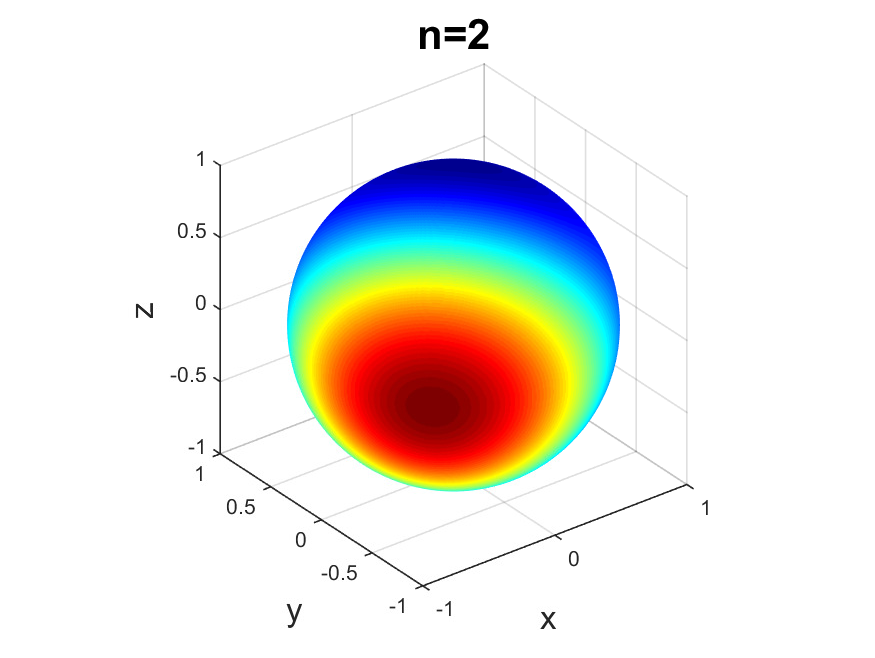
\includegraphics[width=0.4\textwidth]{kugel/Gibbs/GibbsN_2.pdf}
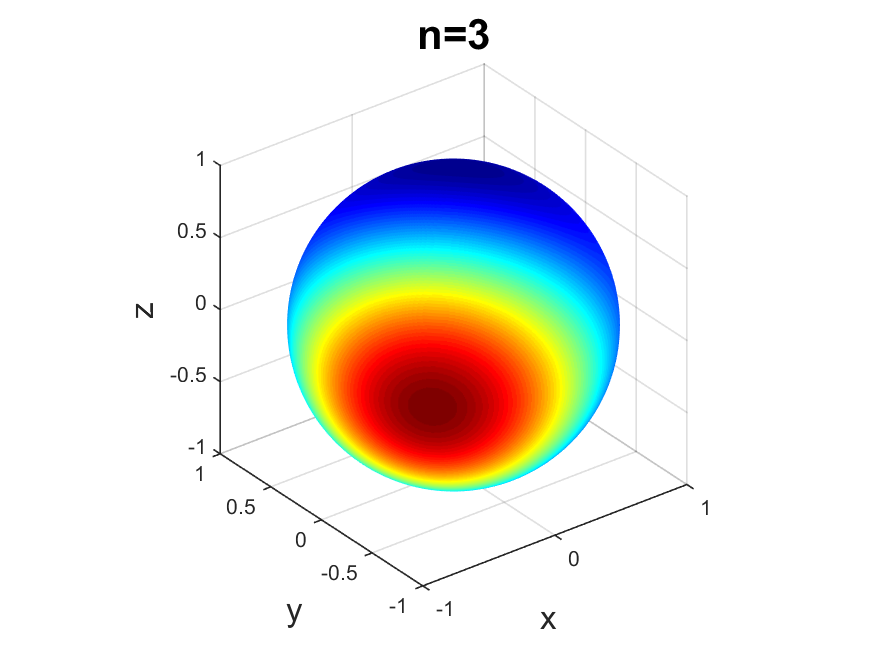
\includegraphics[width=0.4\textwidth]{kugel/Gibbs/GibbsN_3.pdf}
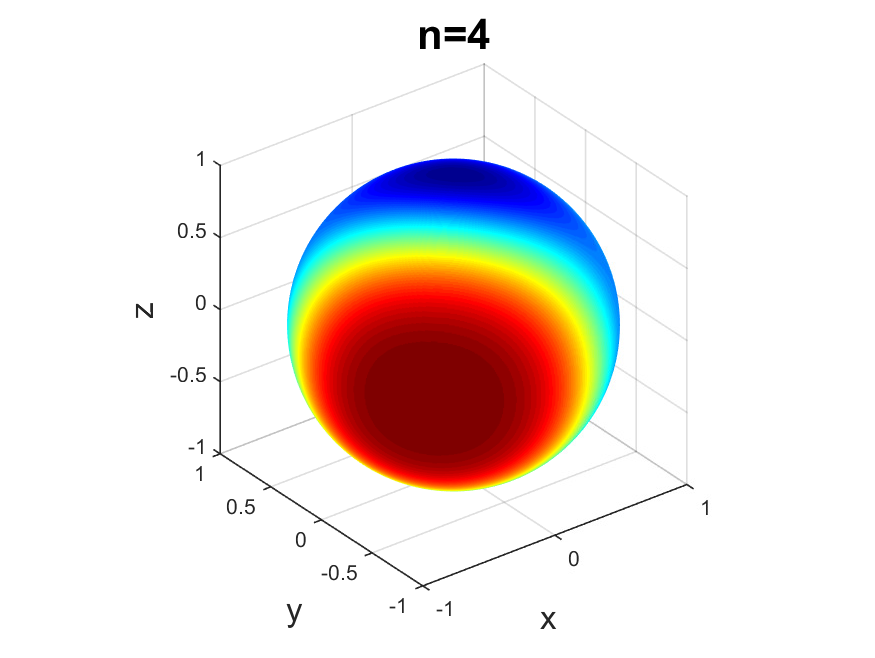
\includegraphics[width=0.4\textwidth]{kugel/Gibbs/GibbsN_4.pdf}
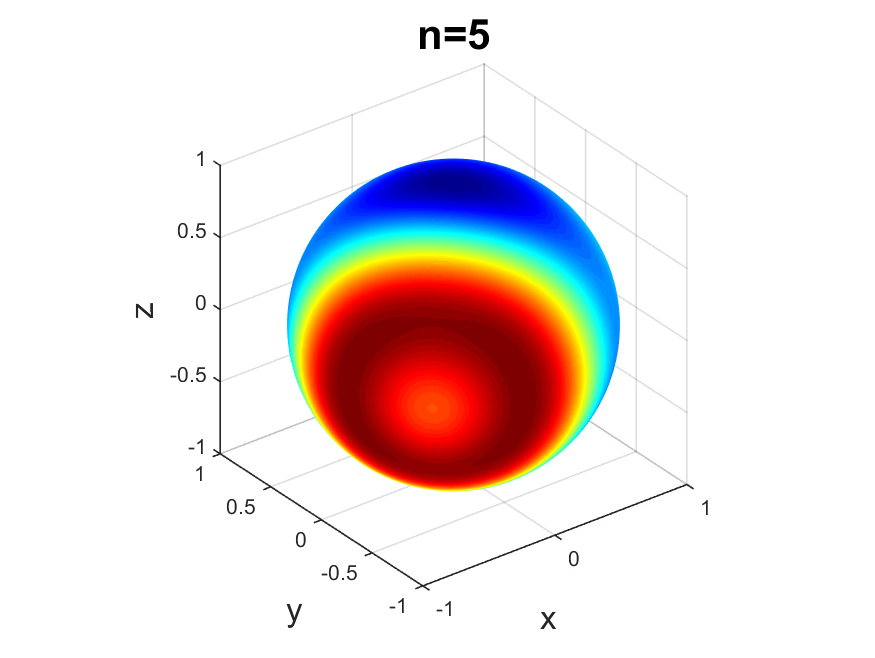
\includegraphics[width=0.4\textwidth]{kugel/Gibbs/GibbsN_5.pdf}
\caption{Gibbsscher-Effekt $n=1$ bis $n=5$
\label{skript:Gibbs1}}
\end{figure}

\begin{figure}% Gibbsscher-Effekt
\centering
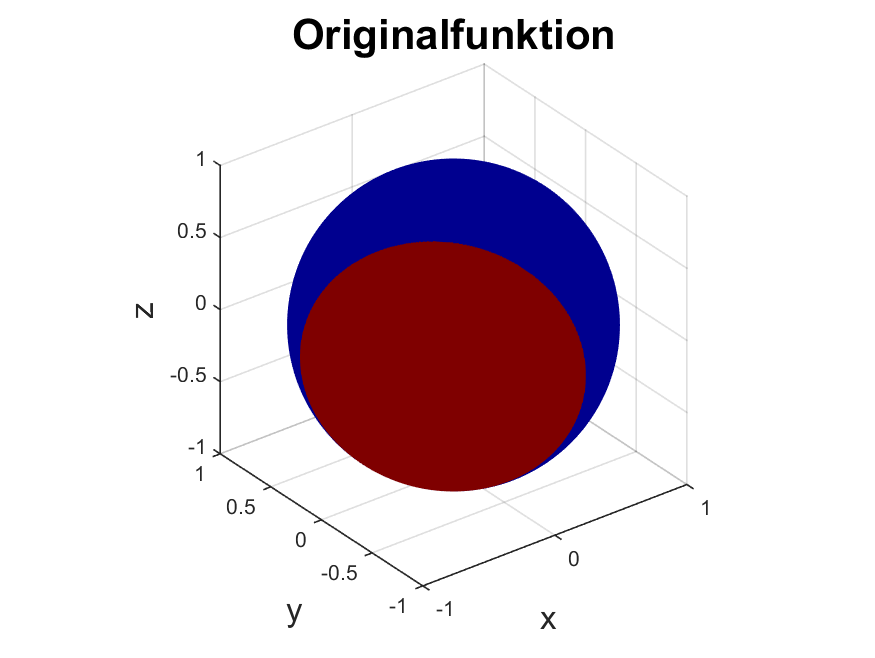
\includegraphics[width=0.4\textwidth]{kugel/Gibbs/GibbsOriginalFunktion.pdf}
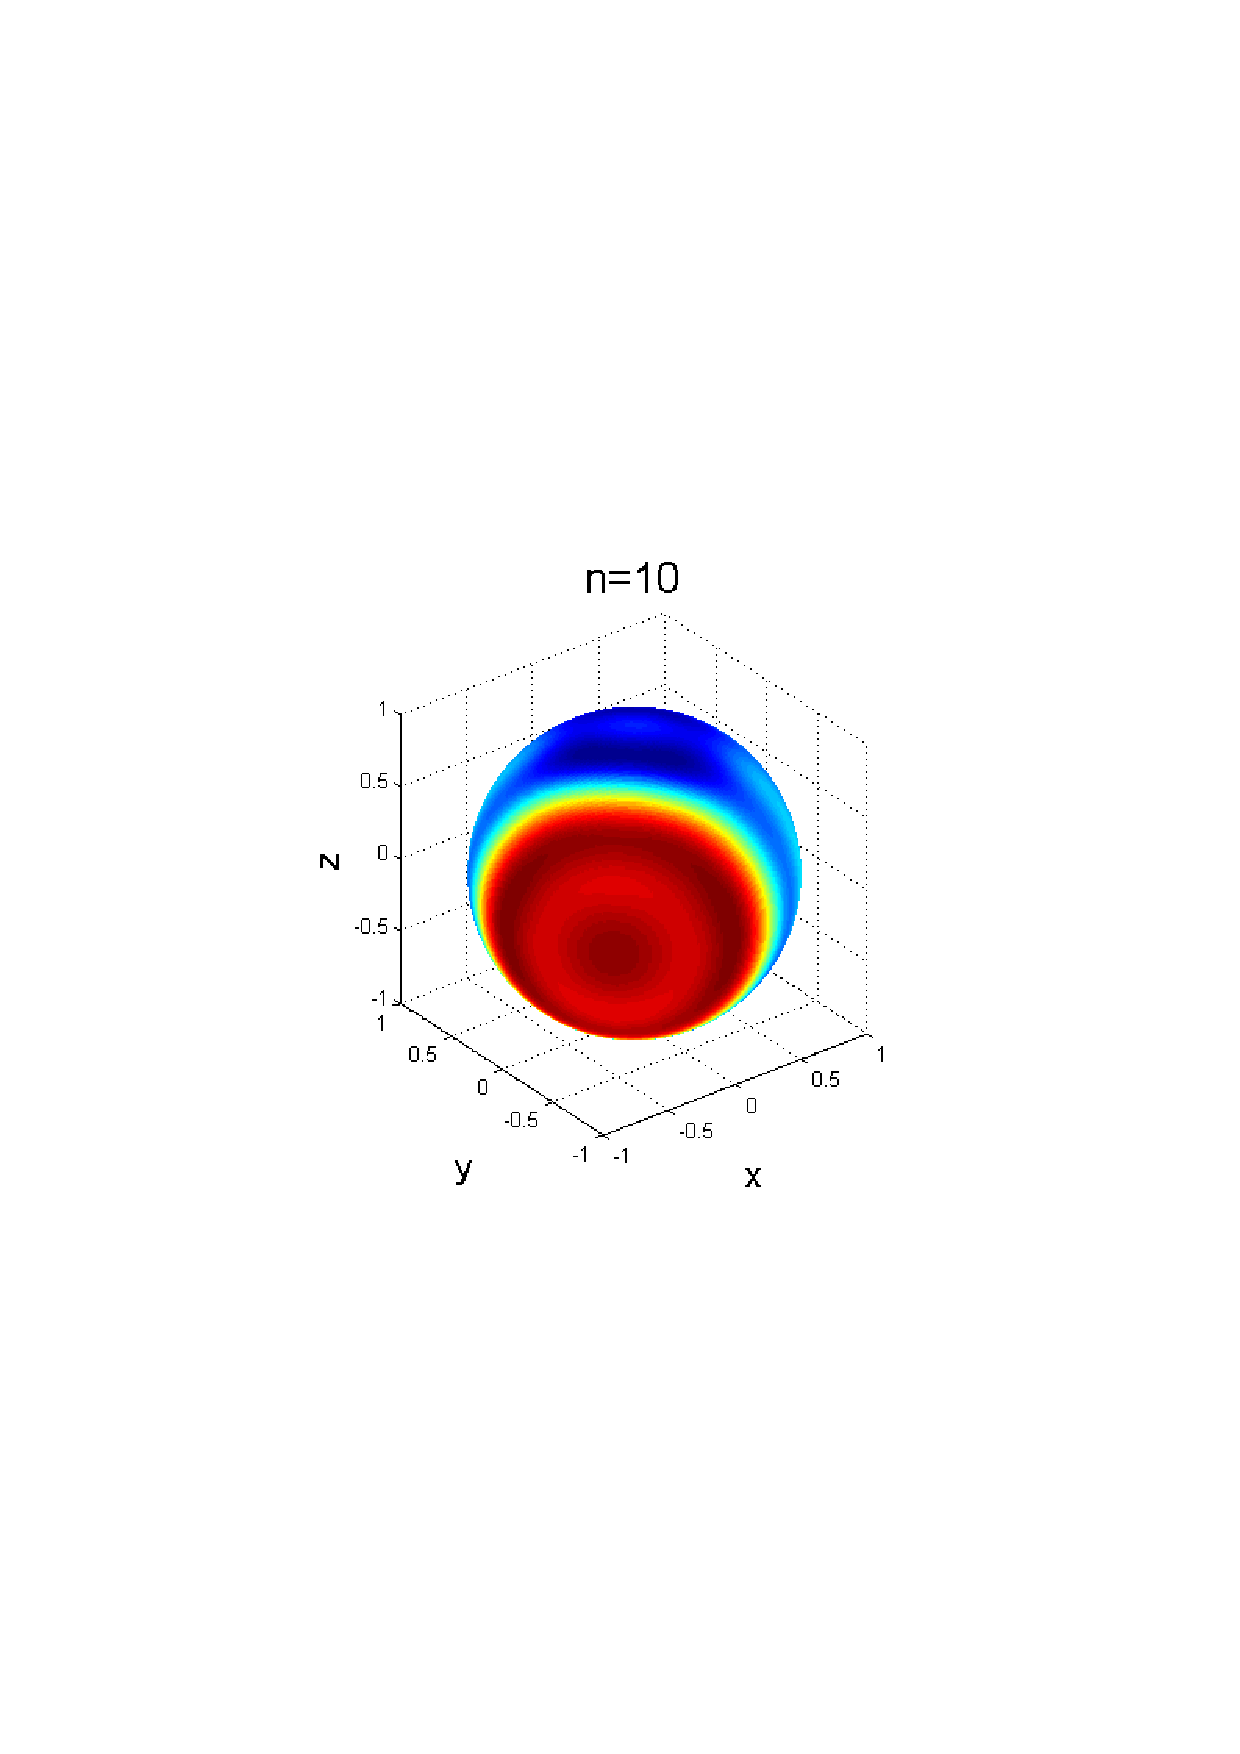
\includegraphics[width=0.4\textwidth]{kugel/Gibbs/GibbsN_10.pdf}
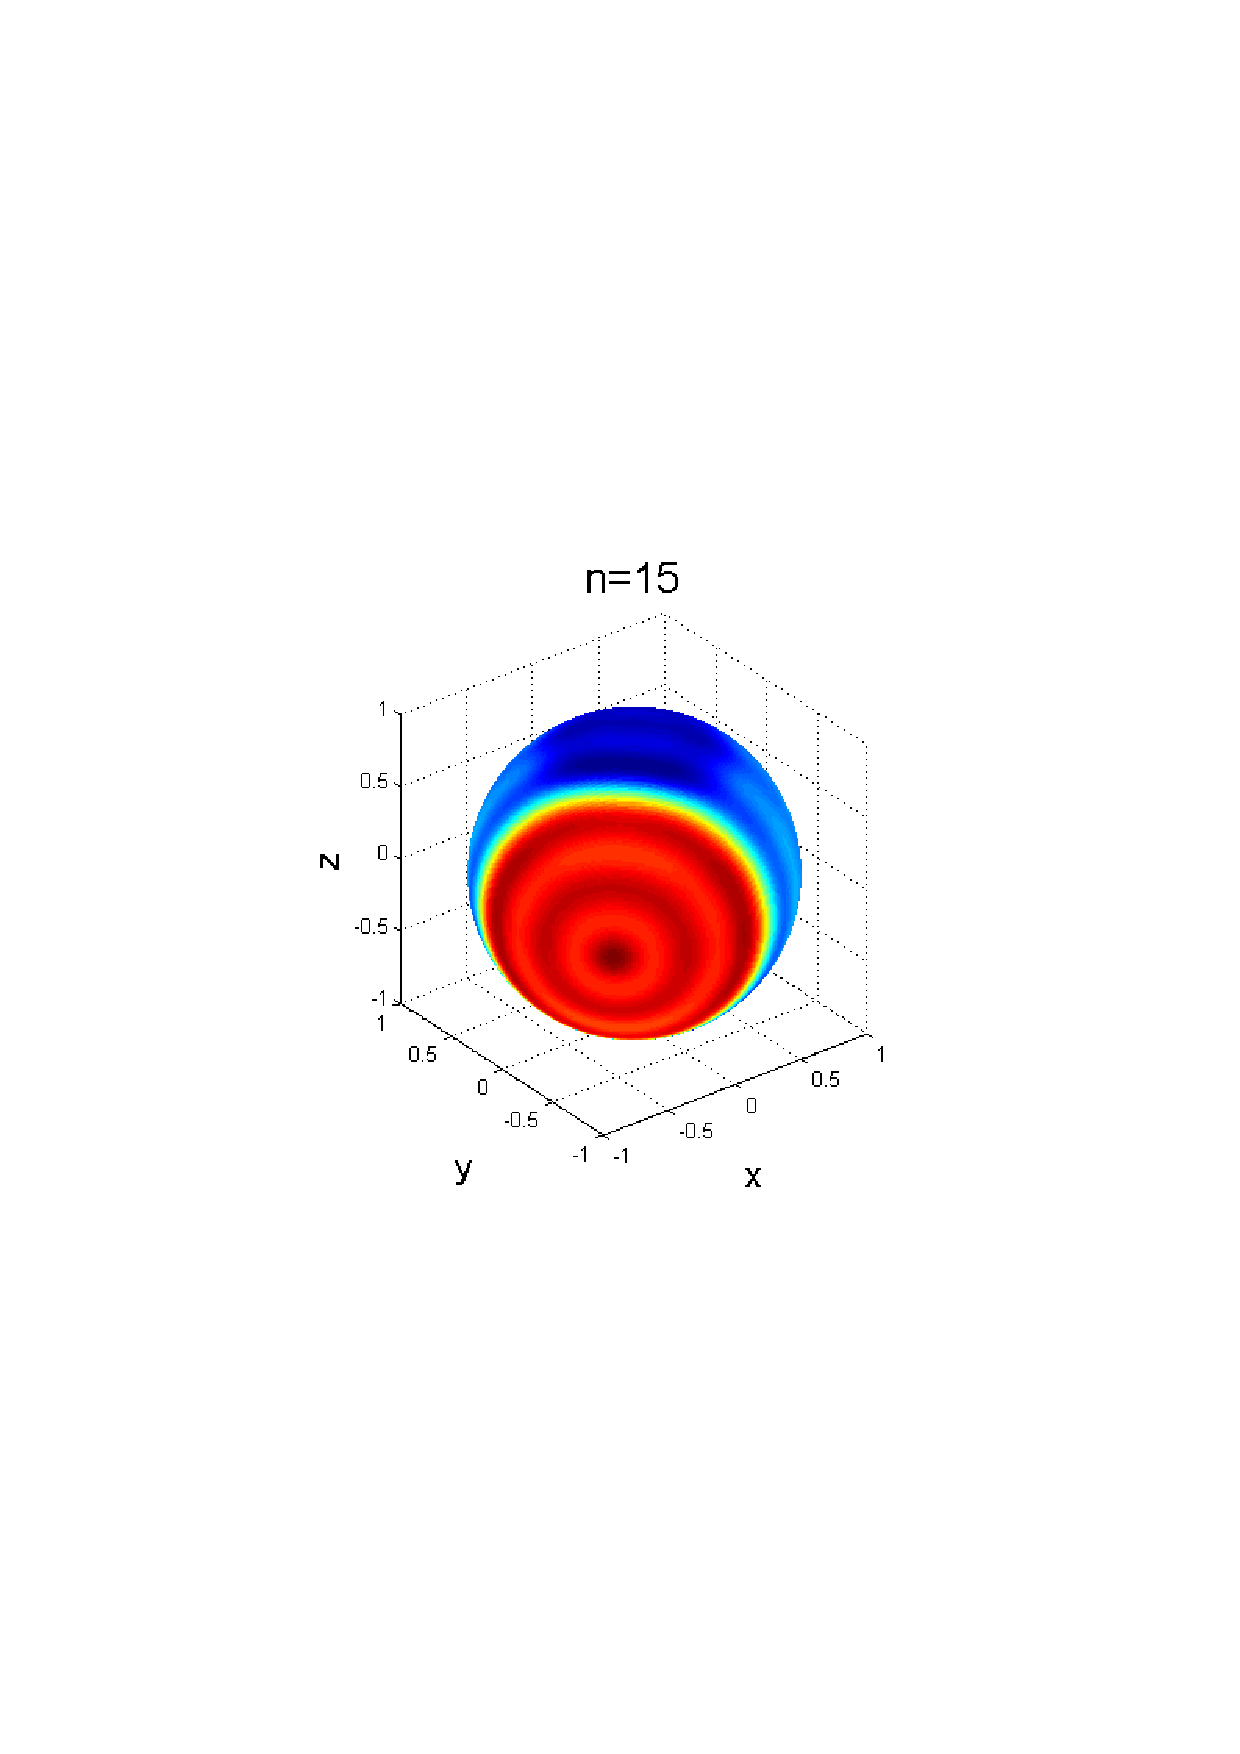
\includegraphics[width=0.4\textwidth]{kugel/Gibbs/GibbsN_15.pdf}
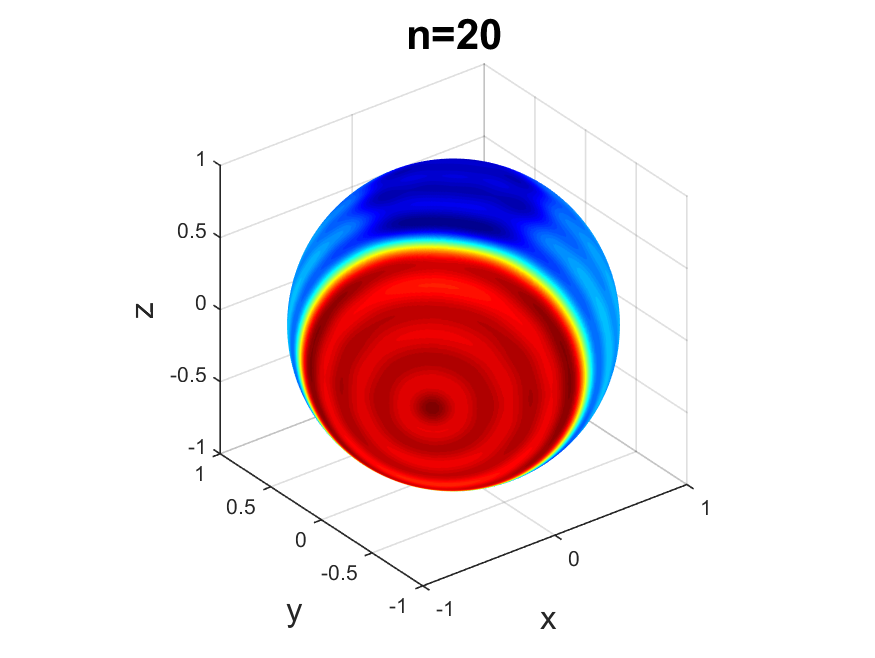
\includegraphics[width=0.4\textwidth]{kugel/Gibbs/GibbsN_20.pdf}
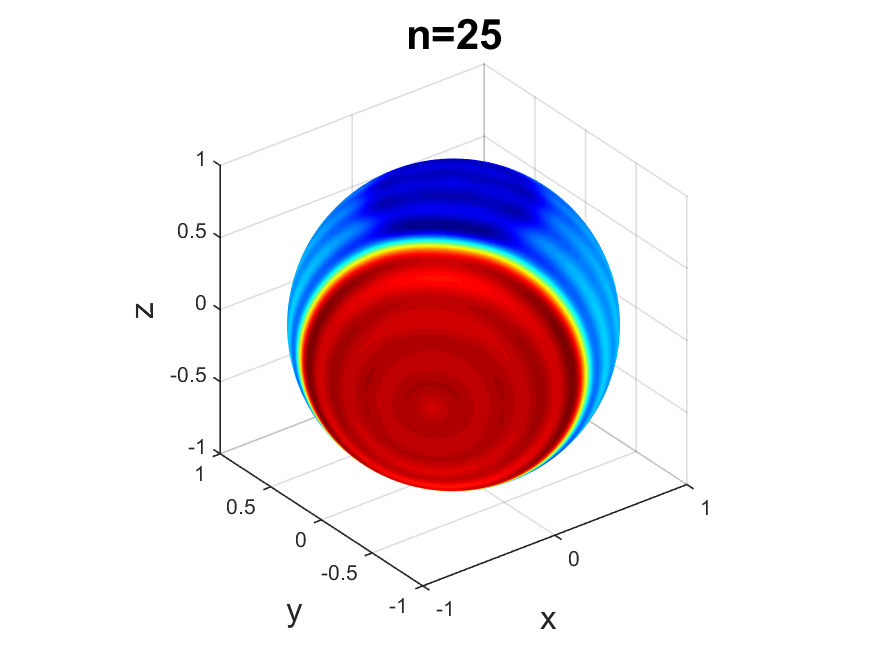
\includegraphics[width=0.4\textwidth]{kugel/Gibbs/GibbsN_25.pdf}
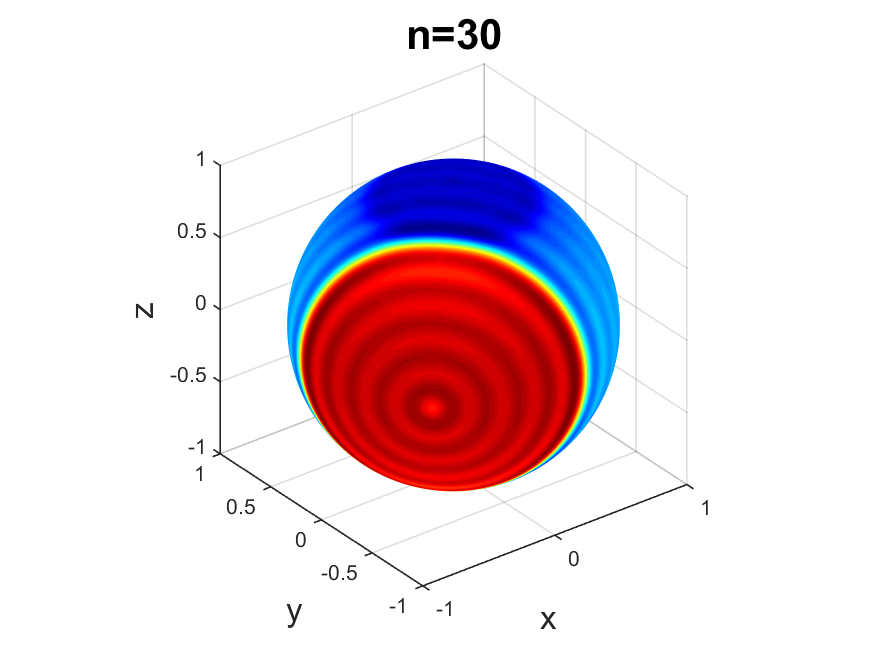
\includegraphics[width=0.4\textwidth]{kugel/Gibbs/GibbsN_30.pdf}
\caption{Gibbsscher-Effekt $n=10$ bis $n=30$
\label{skript:Gibbs2}}
\end{figure}

\section{Quellen}
\rhead{Quellen}

https://de.wikipedia.org/wiki/Kugelkoordinaten


\printbibliography[heading=subbibliography]
\end{refsection}